\subsection{Quickstart}

\begin{verbatim}
import datetime
import geospacelab.datahub as datahub
import geospacelab.visualization.mpl as gsl_mpl
\end{verbatim}

\subsubsection{Swarm Data Access}

\paragraph{Initial settings}

\begin{verbatim}
dt_fr = datetime.datetime(2016, 3, 15, 18, 18)
dt_to = datetime.datetime(2016, 3, 15, 18, 23)
sat_id = "A"
\end{verbatim}

\paragraph{Create a datahub}

\begin{verbatim}
dh = datahub.DataHub(dt_fr=dt_fr, dt_to=dt_to, visual='on')
\end{verbatim}

\paragraph{Dock a Swarm dataset}

Docking a dataset is the process of loading the dataset into the datahub. It is done by calling the \texttt{dock} method of the datahub object. The method takes the name patterns of the dataset as an argument and returns a dataset object.

The following code docks the Swarm MAG LR dataset for the specified time range (shown above) and satellite ID. A full list of the supported datasets and their name patterns can be found in the \href{/supported-datasets}{Supported datasets} tutorial.

\begin{verbatim}
ds = dh.dock(datasource_contents=['esa_eo', 'swarm', 'l1b', 'mag_lr'], sat_id=sat_id, add_APEX=True,)
\end{verbatim}

\begin{verbatim}
Load IGRF coefficients ...
\end{verbatim}

\begin{verbatim}
Searching the data product "MAG_LR" with the version "latest" on the server...
The file [PosixPath('/data/afys -ionosphere/data/ESA/SWARM/Level1b/MAG_LR/0701/Sat_A/2016/SW_OPER_MAGA_LR_1B_20160315T000000_20160315T235959_0701_MDR_MAG_LR.cdf'), PosixPath('/data/afys -ionosphere/data/ESA/SWARM/Level1b/MAG_LR/0701/Sat_A/2016/SW_OPER_MAGA_LR_1B_20160315T000000_20160315T235959_0701_ASM_VFM_IC.cdf')] already exists: skip downloading.
WARNING: Multiple files found for the pattern *20160315T000000*20160315T235959*0701*.cdf in the directory /data/afys -ionosphere/data/ESA/SWARM/Level1b/MAG_LR/0701/Sat_A/2016!
/opt/anaconda3/envs/Swarm/lib/python3.12/site -packages/numpy/_core/numeric.py:476: RuntimeWarning: invalid value encountered in cast
  multiarray.copyto(res, fill_value, casting='unsafe')
\end{verbatim}

\subparagraph{List the variables included in the dataset}

\begin{verbatim}
ds.list_all_variables()
\end{verbatim}

\begin{verbatim}
Dataset: esa/earthonline | swarm | mag | mag_lr
Printing all of the variables ...
|No.                 |Variable name                 |Variable name (Source)        |Description                                                                                         |
| - - - - - - - - - - - - - - - - - - - -| - - - - - - - - - - - - - - - - - - - - - - - - - - - - - -| - - - - - - - - - - - - - - - - - - - - - - - - - - - - - -| - - - - - - - - - - - - - - - - - - - - - - - - - - - - - - - - - - - - - - - - - - - - - - - - - - - - - - - - - - - - - - - - - - - - - - - - - - - - - - - - - - - - - - - - - - - - - - - - - - - -|
|1                   |SC_DATETIME                   |N/A                           |Time of observation                                                                                 |
|2                   |SYNC_STATUS                   |SyncStatus                    |                                                                                                    |
|3                   |SC_GEO_LAT                    |Latitude                      |Geographic Latitude                                                                                 |
|4                   |SC_GEO_LON                    |Longitude                     |Geographic Longitude                                                                                |
|5                   |SC_GEO_r                      |N/A                           |                                                                                                    |
|6                   |B_VFM                         |B_VFM                         |                                                                                                    |
|7                   |B_VFM_x                       |N/A                           |B in x direction of VFM frame                                                                       |
|8                   |B_VFM_y                       |N/A                           |B in y direction of VFM frame                                                                       |
|9                   |B_VFM_z                       |N/A                           |B in z direction of VFM frame                                                                       |
|10                  |B_VFM_x_err                   |N/A                           |                                                                                                    |
|11                  |B_VFM_y_err                   |N/A                           |                                                                                                    |
|12                  |B_VFM_z_err                   |N/A                           |                                                                                                    |
|13                  |B_NEC                         |B_NEC                         |                                                                                                    |
|14                  |B_N                           |N/A                           |B in northward direction of NEC frame                                                               |
|15                  |B_E                           |N/A                           |B in eastward direction of NEC frame                                                                |
|16                  |B_C                           |N/A                           |B in downward direction of NEC frame                                                                |
|17                  |dB_Sun_VFM                    |dB_Sun                        |                                                                                                    |
|18                  |dB_Sun_VFM_x                  |N/A                           |dB due to Sun induced perturbation in x direction of VFM frame                                      |
|19                  |dB_Sun_VFM_y                  |N/A                           |dB due to Sun induced perturbation in y direction of VFM frame                                      |
|20                  |dB_Sun_VFM_z                  |N/A                           |dB due to Sun induced perturbation in z direction of VFM frame                                      |
|21                  |dB_AOCS_VFM                   |dB_AOCS                       |                                                                                                    |
|22                  |dB_AOCS_VFM_x                 |N/A                           |dB due to AOCS induced perturbation in x direction of VFM frame                                     |
|23                  |dB_AOCS_VFM_y                 |N/A                           |dB due to AOCS induced perturbation in y direction of VFM frame                                     |
|24                  |dB_AOCS_VFM_z                 |N/A                           |dB due to AOCS induced perturbation in z direction of VFM frame                                     |
|25                  |dB_other_VFM                  |dB_other                      |                                                                                                    |
|26                  |dB_other_VFM_x                |N/A                           |dB due to all other sources of perturbation in x direction of VFM frame                             |
|27                  |dB_other_VFM_y                |N/A                           |dB due to all other sources of perturbation in y direction of VFM frame                             |
|28                  |dB_other_VFM_z                |N/A                           |dB due to all other sources of perturbation in z direction of VFM frame                             |
|29                  |B_VFM_err                     |B_error                       |                                                                                                    |
|30                  |q_NEC_CRF                     |q_NEC_CRF                     |                                                                                                    |
|31                  |Att_error                     |Att_error                     |                                                                                                    |
|32                  |FLAG_B                        |Flags_B                       |Flag B                                                                                              |
|33                  |FLAG_q                        |Flags_q                       |Flag q                                                                                              |
|34                  |FLAG_Platform                 |Flags_Platform                |Flag Platform                                                                                       |
|35                  |FLAG_B_BIN_AUX                |N/A                           |Binary flag for B                                                                                   |
|36                  |FLAG_B_BIN_IND                |N/A                           |                                                                                                    |
|37                  |FLAG_q_BIN_AUX                |N/A                           |Binary flag for q                                                                                   |
|38                  |FLAG_q_BIN_IND                |N/A                           |                                                                                                    |
|39                  |FLAG_Platform_BIN_AUX         |N/A                           |Binary flag for Platform                                                                            |
|40                  |FLAG_Platform_BIN_IND         |N/A                           |                                                                                                    |
|41                  |FLAG_F                        |Flags_F                       |Flag F                                                                                              |
|42                  |FLAG_F_BIN_AUX                |N/A                           |Binary flag for F                                                                                   |
|43                  |FLAG_F_BIN_IND                |N/A                           |                                                                                                    |
|44                  |ASM_Freq_Dev                  |ASM_Freq_Dev                  |                                                                                                    |
|45                  |F                             |F                             |Magnetic field intensity                                                                            |
|46                  |F_err                         |F_error                       |                                                                                                    |
|47                  |dF_Sun                        |dF_Sun                        |                                                                                                    |
|48                  |dF_AOCS                       |dF_AOCS                       |                                                                                                    |
|49                  |dF_other                      |dF_other                      |                                                                                                    |
|50                  |SC_APEX_LAT                   |N/A                           |APEX Latitude                                                                                       |
|51                  |SC_APEX_LON                   |N/A                           |APEX Longitude                                                                                      |
|52                  |SC_APEX_MLT                   |N/A                           |APEX Magnetic Local Time                                                                            |
|53                  |SC_GEO_LST                    |N/A                           |Local Solar Time                                                                                    |
\end{verbatim}

\subparagraph{Get a variable and data array}

\begin{verbatim}
B_N = ds['B_N']
\end{verbatim}

Above returns a GeospaceLAB Variable object. To get the data array, call

\begin{verbatim}
B_N_arr = B_N.value
\end{verbatim}

Above returns a \texttt{numpy.ndarray} data array.

\subsubsection{Swarm Data Visualization}

The following example shows how to make the time series plots in GeospaceLAB with the Swarm MAG LR data. More examples can be found in \href{/example-swarm-mag}{Examples}

\begin{verbatim}
# Create a figure
fig = gsl_mpl.create_figure(figsize=(8, 12))
# Add a time series dashboard to the figure
db = gsl_mpl.dashboards.TSDashboard(figure=fig, dt_fr=dt_fr, dt_to=dt_to)
# Set the panel layouts in the dashboard. 
# The layout is a list of lists, where each inner list represents a row of panels in the dashboard. 
# Each element in the inner list is a variable from the dataset that will be plotted in that panel.
# This allows for flexible arrangement of multiple plots in a single dashboard.
# To add or remove a panel, simply modify the inner lists accordingly. 
# For example, to remove the first panel, simply remove the first inner list: panel_layouts = [ [ds['B_N'], ds['B_E'], ds['B_C']], ... ]
panel_layouts = [
    [ds['F']],
    [ds['B_N'], ds['B_E'], ds['B_C']],
    [ds['B_VFM_x'], ds['B_VFM_y'], ds['B_VFM_z']],
    [ds['dB_Sun_VFM_x'], ds['dB_Sun_VFM_y'], ds['dB_Sun_VFM_z']],
    [ds['dB_AOCS_VFM_x'], ds['dB_AOCS_VFM_y'], ds['dB_AOCS_VFM_z']],
    [ds['dB_other_VFM_x'], ds['dB_other_VFM_y'], ds['dB_other_VFM_z']],
    [ds['FLAG_F_BIN_AUX']],
    [ds['FLAG_B_BIN_AUX']],
    [ds['FLAG_q_BIN_AUX']],
    [ds['FLAG_Platform_BIN_AUX']],
]
db.set_layout(panel_layouts)
# Plotting the data in the dashboard
db.draw()
# Add panel labels to the dashboard
db.add_panel_labels()
# Add a title to the dashboard
db.add_title(y=1.02,title='Swarm -{} MAG LR Zoom'.format(ds.sat_id), fontsize='medium', append_time=True)
# Show the figure/dashboard
db.show()
\end{verbatim}

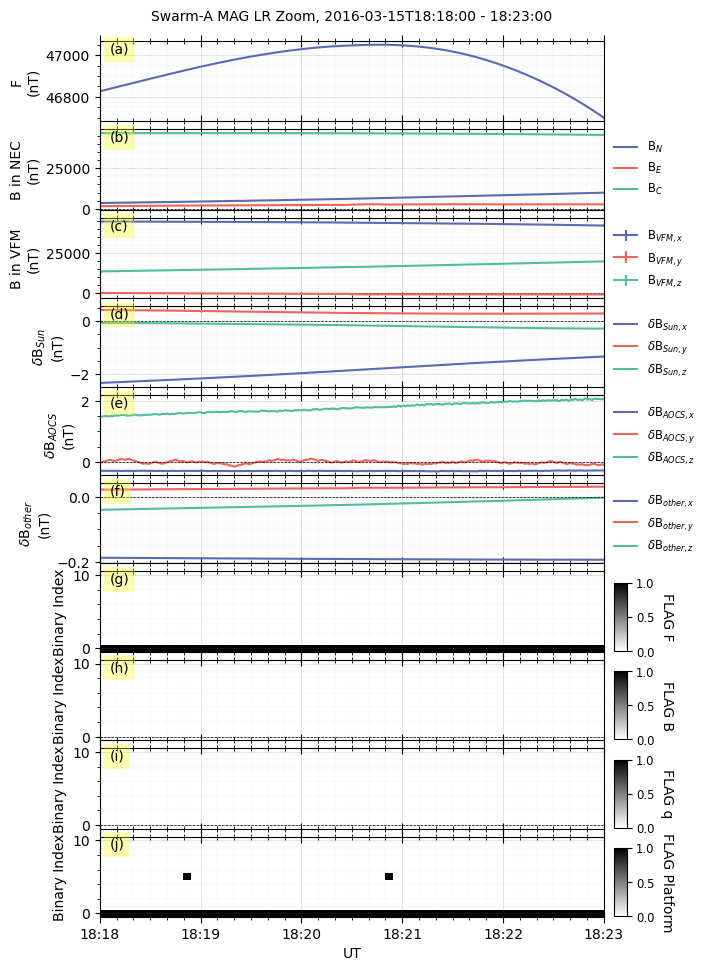
\includegraphics[width=0.7\linewidth]{files/a215a1b350897a52e3808de731f33756.png}